\begin{frame}{\texttt{keybert}}
Librairie Python qui exploite les plongements de mots BERT pour générer des mots\customhyphen/phrases-clés les plus similaires à un document.
   \begin{figure}[!ht]
        \centering
        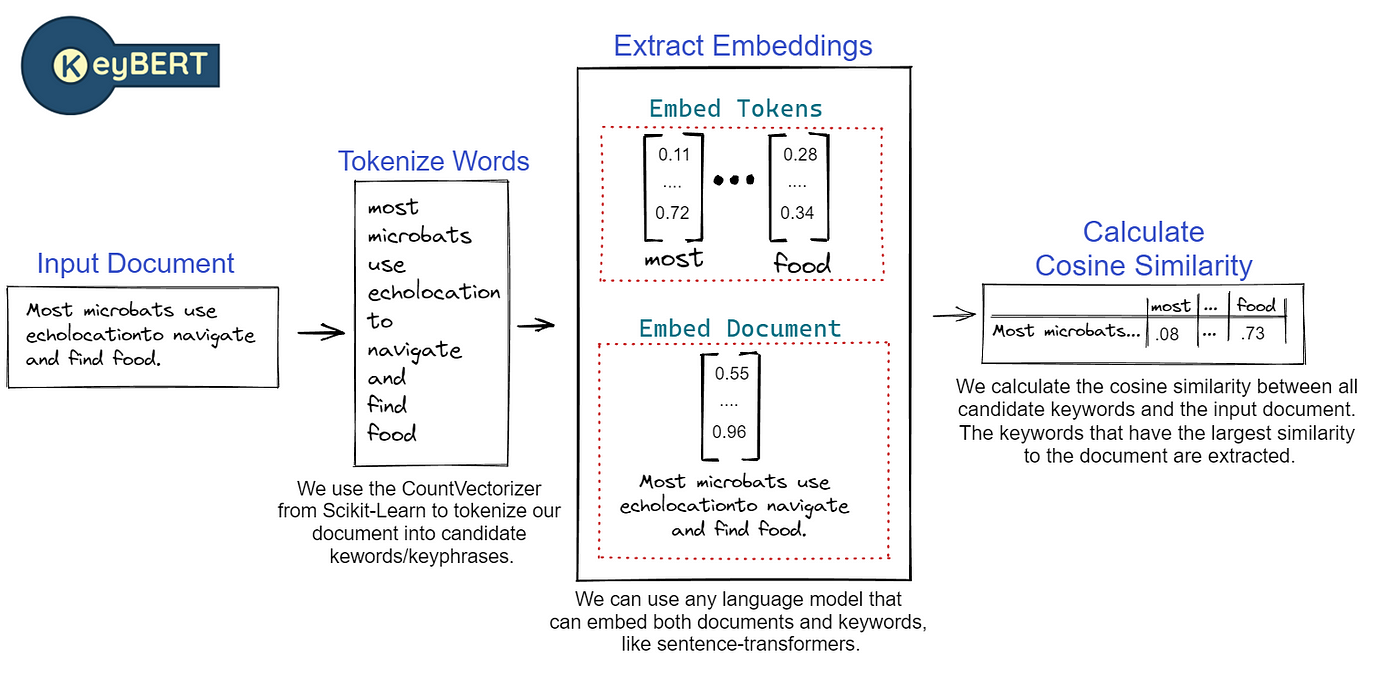
\includegraphics[width=110mm,scale=0.5]{pic/keybert.png}
        \caption{\textit{Pipeline} de la librairie \texttt{keybert} \citep{grootendorst2020keybert}.}
        \label{fig:enter-label}
    \end{figure}
\end{frame}
\begin{frame}{Améliorer les sorties de \texttt{keybert}}
Limitations de \texttt{keybert} :
\begin{itemize}
\item on doit spécifier la longueur (optimale) des n-grammes à extraire
\item la grammaticalité des phrases n'est pas prise en compte
\begin{itemize}
p. ex. \textit{spinal les muscles}
\end{itemize}
\item mots très similaires dans la liste des mots-clés 
% Temporarily remove bullet points for this itemize environment
\begingroup
\setbeamertemplate{itemize items}{}
\begin{itemize}
\item \textit{réflexes tendineux} sont, 0.468
\item les \textit{réflexes tendineux}, 0.4615
\end{itemize}
\endgroup
\end{itemize}

Alternative : réglage fin des sorties
\begin{itemize}
\item diversification des résultats : \textit{Maximal Marginal Relevance}
\begin{itemize}
\item \og{}pertinence marginale maximale\fg{} : combinaison linéaire de la pertinence par rapport à la requête et la nouveauté
\item un document a une PMM s'il répond à la requête et contient peu de similarité avec les documents précédents \citep{boutin2006biais}
\end{itemize}
\item préservation de la grammaticalité de la phrase (motifs POS) \\$\rightarrow$ {\small\texttt{keyphrase-vectorizers}} {\small\citep{schopf22}}
\end{itemize}
\end{frame}
